\section{Suit2p pipeline}
\label{sec:Suit2ppipeline}

%You will need to analyze imaging data from large numbers of neurons. You will first need to identify  the cells in the images and extract their fluorescence traces. We have our own code, but you might use something like this:

The recordings from two-photon microscopy and calcium indicators yield the observation of large neuron populations' activity that must be processed in a suitable way to extract neuron's fluorescence traces. This data comprises multi-plane movies of a great number of cells, depending on the imaged region. Computational methods for its treatment should be not only accurate, but fast, as to grant the feasibility of substantial data's processing. 
\\In this project, the \textit{Suite2p} pipeline was used. This set of algorithms implements four modular processing independent steps: Image registration from raw movies through time and spatial phase correlation, the detection of regions of interest (ROIs), their interactive labelling and quality control and finally the extraction of a single representative fluorescence signal for each ROI.

The first stage of Suit2p is image registration, spatially aligning images taken at different times or from different viewpoints. This step from the algorithm was not used, as it was found to not perform as well as the iterative registration method described above for our data set. 

In much similiarity, the algorithm receives raw movies as inputs and corrects for the effects of brain movement. 
This registration is also based on finding a correlation-peak between a frame and a target image with a fast fourier transform, determining its offset, and applying the appropriate shift by means of FFT-based interpolation.
Additionally, to emphasize high-frequency content such as somata calcium-filled cellular compartments that could be dominated over in the previous scheme, the algorithm uses phase correlation, firstly spatially whitening the images - decorrelating the spatial information and leaving it with variance one - and then computing its correlation-maps. Sub-pixel shifts are also detected and corrected by an extension of this principle.
Non-rigid and rotation alignments are also made possible, by means of a generated globally non-rigid transformation. [TAKE THIS OUT]

The second stage uses the aligned movies and selects spatial regions of interest (ROIs) - somata, dendrites, spines or butons - with each pixel assigned to a positive weight. The model assumes the origin of the recorded signal in each pixel to be coming from three possible origins: the actual ROIs, measurement noise, but also from the neuropil - synaptically dense regions, out-of-focus dendrites and axons whose average activity contaminates the detection with a large and diffuse signal. 

To account for this important effect, the neuropil signal is represented in a set of spatially-localized basis functions \textbf{B}, covering the full field of view and each pixel \textit{k}. In each basis function j, the neuropil signal is a smooth timecourse $\vec{n}_{j}(t)$. Assuming the ROI signals to also be spatially localized, and having that, for each ROI i, its pixels all follow the same time course $\vec{f}_i(t)$ which is scaled by a constant positive factor, given by a sparse matrix $\Lambda _{ki}$ that is null if the pixel k does not belong to the ROI i. Finally, the noise is taken to be Gaussian and described by $\vec{\eta} _k(t) \sim N(0, \sigma ^2)$. We obtain the final model for the recorded signal $\vec{r}_k$(t) at pixel k:

\begin{equation}
    \vec{r}_k(t)=\sum_i \Lambda _{ki} \vec{f}_i (t) + \sum _j B_{kj} \vec{n}_j(t) + \vec{\eta}_k(t)
\end{equation}

This model is thereupon fitted to the data, by iterations of ROI detection (finding new sources), activity extractions (re-estimating time courses and neuropil contribution) and pixel-reassignments (taking into account the other ROIs, reestimating a given ROI spatial distribution).

The third stage amounts to the quality control of the classification, distinguishing between cell and non-cell (compartments, such as dendrites or axons), and lowering the fluorescence variance in each ROI. This is firstly done by an automated classifier and then curated by the used through the software's GUI that displays an improved resolution image, each ROIs information,  and allows its relabelling as cell/non-cell. One of the great advantages of this pipeline is that the selection-stage improves with use and training of the classifier. The implemented classifier is based on a set of $k$ feature statistics $r_k(n)$ computed for each ROI $n$ (encompassing both activity and shape parameters). The distributions of these features are estimated by human-labelled data and then fed to a Bayes classifier that is trained to reproduce them. The classifiers' cell $p^+_k(x)$ versus non-cell $p^-_k(x)$ smoothed empirical distributions for each statistic $x$ are then applied to new data cells. A new ROI N is classified by comparing every combined statistics' cell score $\prod_k p^+_k(r_k(N))$ with its non-cell score $\prod_k p^-_k(r_k(N))$, and labelling it cell or no-cell according to the category that results in the highest score for that ROI.

\begin{figure}[H] \centering 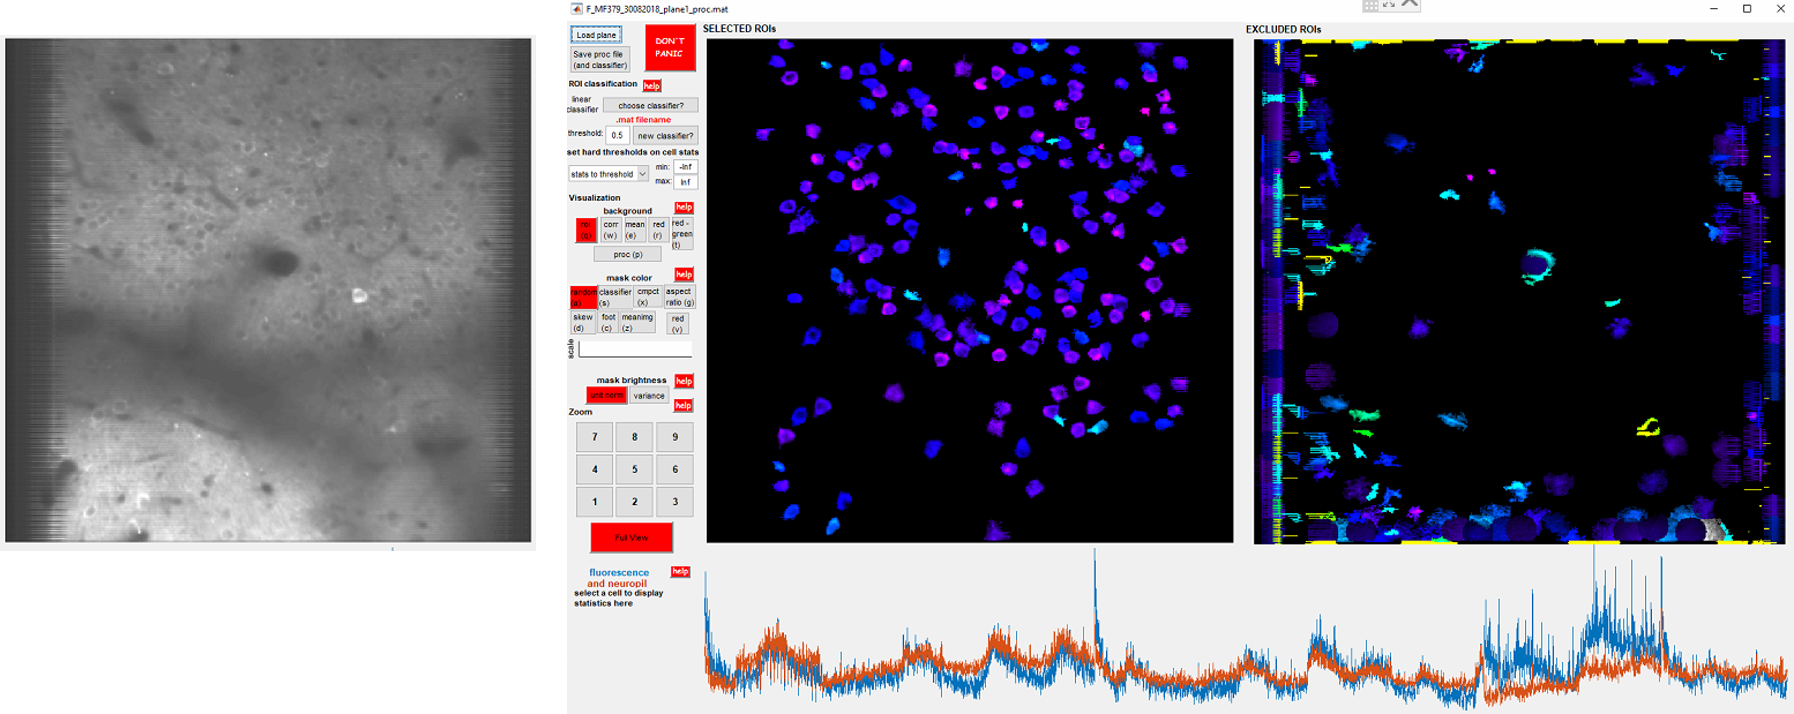
\includegraphics[width=13cm,height=13cm,keepaspectratio]{Figures/7.Results/ftraces/suit2p.png} 
%\caption{6_popPlots_Animal2_Session6} 
\end{figure}

Finally, the fourth stage of the pipeline outputs, for each ROI, a single calcium fluorescence time-varying signal. Again, this signal is corrected for the neuropil contamination signals. Furthermore, the spike train - the action potential sequence - that causes this signal is estimated, by use of a fitting model. 
A model is used for the uncorrected fluorescence $\vec{F}_i$, with a contribution by the convolution of the spike train $\vec{s}_i \geq 0$ with the calcium response kernel $\vec{k}_i$, a scalled neuropil and the noise:

\begin{equation}
    \vec{F}_i(t) = [\vec{s}_i * \vec{k}_i](t) + c_i \vec{N}_i (t) + noise
\end{equation}

To fit this model, $\vec{F}_i$ is extracted for each ROI i, the neuropil trace $\vec{N}_i$ is computed by averaging pixels in a ring shaped region around the ROI, and finally the coefficient $c_i$ and the spike train $\vec{s}_i$ are estimated for each cell by optimization of the cost function:

\begin{equation}
    Cost(\vec{s}_i, c_i)=||\vec{F}_i - \vec{s}_i * \vec{k}_i - c_i \cdot \vec{N}_i|| ^2 + \lambda \cdot L(\vec{s}_i)
\end{equation}

with $L(\vec{s}_i)$ a continuous, non-negative possible penalty on the spike train for each ROI.

In this way, the \textit{Suit2p} treatment of the raw movies produces a neuropil-corrected calcium trace $\vec{F}_i - c_i \vec{N}_i$, as well as the spike times estimates $\vec{s}_i$.

This processed data of fluorescence traces will be the substance for the posterior analysis.